% Intended LaTeX compiler: pdflatex
\documentclass[11pt]{article}
\usepackage[utf8]{inputenc}
\usepackage[T1]{fontenc}
\usepackage{graphicx}
\usepackage{grffile}
\usepackage{longtable}
\usepackage{wrapfig}
\usepackage{rotating}
\usepackage[normalem]{ulem}
\usepackage{amsmath}
\usepackage{textcomp}
\usepackage{amssymb}
\usepackage{capt-of}
\usepackage{hyperref}
\documentclass{article}
\addtolength{\voffset}{-2.25cm}
\usepackage[document]{ragged2e}
\usepackage{fancyhdr}
\pagestyle{fancy}
\fancyhf{}
\lhead{Minor scales and modes for ii-v-i progressions}
\rhead{Bartev - 2020-12-28}
\author{Bartev Vartanian}
\date{2021-03-28}
\title{Minor scales and modes for ii-v-i progressions}
\hypersetup{
 pdfauthor={Bartev Vartanian},
 pdftitle={Minor scales and modes for ii-v-i progressions},
 pdfkeywords={},
 pdfsubject={},
 pdfcreator={Emacs 27.1 (Org mode 9.3)}, 
 pdflang={English}}
\begin{document}

\maketitle


\section*{Minor ii-v's in Bb}
\label{sec:org97f04c6}

See Softly in the Morning Sunrise for an example

ii-7b5 (C half diminished)

Pianists may voice this differently (below)

Maybe a natural 9 on top (debate about this)

\begin{center}
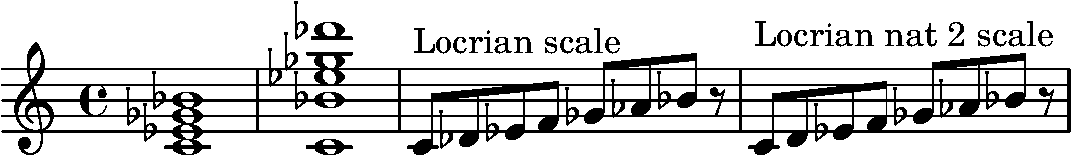
\includegraphics[width=.9\linewidth]{min_ii_v_Bb.pdf}
\end{center}

\section*{Dominant chord (V7b9)}
\label{sec:org4835729}

Will typically play a b13 (b6), in this case the Db

So, the nat 9 from Cm7b5 -> Db adds chromatic motion

\begin{center}
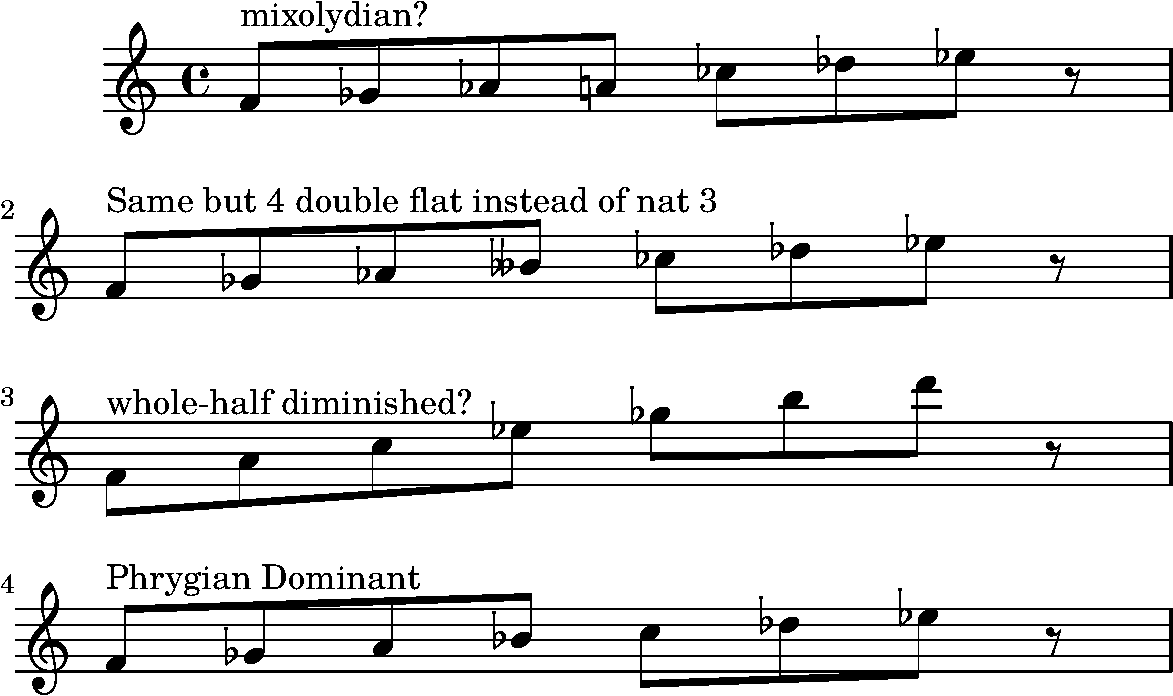
\includegraphics[width=.9\linewidth]{min_ii_v_Bb-dom.pdf}
\end{center}
\end{document}
